% main.tex, to be used with thesis.tex
% This contains the main work of your thesis.

%\bibliography{thesis}  % uses the references stored in Chapter1Radar.bib

\chapter{Experimental Results: Correct Behavior and Performance}

As discussed in the previous chapter, the implementation of a data persistence
layer for NetBEAMS followed the requirements defined in Chapter 4 in regards
to the classification of the SF-BEAMS sensor network and the software
infrastructure provided by the Data Sensor Platform. The implementation was
developed using the infrastructure provided by the online version-control
system repository from NetBEAMS, whose documentation is detailed in Section
\ref{sec:dsp-data-persistence-implementation}.

This chapter details the experiment setup designed to evaluate the
proposed implementation, showing the measurement results collected from the
simulation log and based on the user experience while reusing the collected
data. The pertinent discussion of this work is divided up into different
sections, each of them analyzing different aspects related to data persistence
for NetBEAMS, among others.

\section{Experiment Setup}

The experiment was designed to support different scenarios of regular use of
the mongoDB system infrastructure, simulating the activities of data collection
from the SF-BEAMS network using the NetBEAMS infrastructure. First, the setup
for the data collection of randomly generated data was implemented, which
directly uses already existing NetBEAMS classes. The CRUD scenarios were
implemented in different programming languages, from the data insertion
scenario using the Java Programming Language, to the remaining operations using
the Javascript Scripting language \cite{javascript} and the Python Programming
Language \cite{python}. Similarly, an open-source web application, developed
in the Ruby Programming language \cite{ruby}, was also used. The experiment
scripts were written using Shell Bash Script Language \cite{bashshell} and is
responsible for orchestrating the execution of one single experimental ``run''.

In order to evaluate the DSP Data Persistence component, experiments were
conducted using the DSP Mouse Actions component, a software sensor simulator
that captures the actions performed by the mouse pointer.

\subsection{Experiments Artifacts}

Different artifacts were created to perform the different experiments regarding
the CRUD operations. The ``Create'' operation' was developed in Java, isolating
the services provided by the class DSPMongoCRUDService (Listing
\ref{file:dsp-mongo-service}). It is responsible for the connection handling
with mongoDB, as well as the insertion operation from NetBEAMS. As described
\cite{netbeams-dsp-architecture}, the current version of NetBEAMS supports the
data collection for the YSI Sonde device \cite{YSI-Sonde}, among others used
for demo purposes. After evaluating the database with the YSI Sonde data
handler, the use of the demo component DSP Mouse Actions was used. It captures
the mouse pointer activities performed over a window, for example, mouse clicks
and mouse grag over coordinates x and y.

In order to exercise mongoDB with the same data collected from NetBEAMS, the
existing Java class TestSondeData (Listing
\ref{file:random-ysi-data-generator}), was refactored to provide a random
instance generator for the YSI Data handler implemented in the Java class
SondeDataType (Listing \ref{file:main-ysi-data-handler}). When the Insert
function is executed, the created instances are transferred from the JVM to
the mongoDB, and stored in the collection ``SondeDataContainer''. Specific
details about the execution of mongoDB are depicted in Section
\ref{sec:mongodb-deployment}. Finally, the implementation of the experiment
in the Java class DSPMessageToMongoDBExperiment (Listing
\ref{file:experiment-dsp-java-executor}) was responsible for managing the
creation and insertion of any workload composed by instances of the class
SondeDataType in a bulk manner.

Similarly, the support for the Retrieve, Update and Delete operations against
the inserted workload were implemented using Javascript, as shown in Listing
\ref{file:experiment-scenarios}, respectively by the function calls ``find'',
``update'' and ``remove'' over the collection ``SondeDataContainer''.
Similarly, in order to implement a customizable export system that converts
from mongoDB into the format OpenDAP, a simpler prototype script was developed
in Python, as shown in Listing \ref{file:experiment-export-python}. As a result
of the execution of this script, the exported artifact has the same format as
described in Listing \ref{file:rtc-ysi-opendap}. 

On the other hand, the execution of the main experiment shell script requires
the user to provide the size of the workload, as shown in listing
\ref{cmd:run-persistence-experiment}.

\subsection{Used Workload}
\label{sec:workload}

The workload selected for the experiments reflects the current use of the
collected data at the SF-BEAMS infrastructure. In this way, the experiment
runs for 5 different times to investigate different scenarios. This number is
related to the total number of sensor devices reported to be in operation, as
discussed in Section \ref{sec:sfbeams}. The volume of the workload prepared
after the experiment setup is as follows:

\begin{itemize}
  \item \textbf{First Round}: 483,840 documents, worth of production of the 
  YSI Sonde device during one year, at the rate of 1 observation per minute;
  \item \textbf{Next Rounds}: 483,840 * 4, or 2,419,200 documents, representing
  5 different YSI devices similar to the first round.
\end{itemize}

\subsection{System Environment}

Two different system environments were prepared: one for the External Storage
environment, or Single Server; and another for the Data-Centric Storage, or
Distributed Server. Since the single server is a regular centralized database
system, mongoDB just requires the execution of the database process ``mongod'',
which is started by specifying the directory where the inserted data will be
managed. The distributed server setup requires a different list of processes
(see Section \ref{sec:mongodb-user-experience}): one ``mongod'' process for
each mongoDB shard running on the different mongoDB cluster, one ``mongod''
process to manage the cluster metadata, and one ``mongos'' process, which is
the main one responsible to orchestrate the cluster. The single system
environment is symmetric to the External Storage used to persist the collected
data, while the clustered one simulates the Data-Centric Storage one.

The simulation of both the single and distributed system used both a Mac OS 10
Snow Leopard 64bit, with a total of 8GB of physical memory. However, in order
to simulate different shards in different machines, the use of a VirtualBox
\cite{virtualization} provided the use of guest operating systems to run and
act as the mongoDB shards. In this way, two different versions of the Ubuntu
Linux were used: one 8.04 32bits and another 9.04 64bits. The configuration
used for the single server only uses the process ``mongod'' to be started,
while the clustered setup must be enabled in the database, as in Section
\ref{sec:experiments-setup-single-distributed}.

\subsection{Planned Scenarios}
\label{sec:exp-scenarios}

In order to verify the feasibility of the solution proposed, all CRUD
operations were exercised through the implementation of the practical
scenarios based on the use cases described in Section \ref{sec:use-cases}. In
brief, the use cases were chosen to run with random values such as follows:

\begin{itemize}
  \item (R0) Insert a volume of collected data from sensors using NetBEAMS
  service compatible with 1 year of observations;
  \item (R1) Find all documents whose observations were collected between two
  different dates, say the days between December 8 and 15 of 2009;
  \item (R2) Find all documents whose observations were collected from a given
  known sensor device such as one whose IP address is equals to "192.168.0.102";
  \item (R3) Find all documents whose observations contained specific values
  read from the environment, say Salinity equals to 0.01 and the water temperature
  equals to 46.47;
  \item (U1) Update all the documents whose observations were collected during
  the day of December 2nd, 2009, by adding a tag = ``oil spill'';
  \item (D1) Remove all the documents whose observations were collected on
  December 7th, 2009.
  \item (R4) Export the produced data of the week to CSV files, using the same
  tabular format sequence used in the files distributed by SF-BEAMS using the 
  the OPeNDAP format, as in Listing \ref{file:rtc-ysi-opendap}.
\end{itemize}

\section{Measurement Results}
\label{sec:exp-measurements}

As described in the previous section, the design of the experiments were based
on the specifications of a data persistence for NetBEAMS, using the mongoDB
database system. After setting up the experiment environment, the execution of
the workload was performed against the mongoDB database using its mechanisms
used to manipulate the data generated. It uses the programming language
abstraction to provide access and modifiy the data collected from the NetBEAMS
component. For this reason, this section details these mechanisms used to
implement each of the scenarios defined in the previous section, associating
numerical response time collected from the logs.

\subsection{Insert Operation}

The first set of measurements collected were the ones regarding the use case
R1, shown in Listing \ref{file:dsp-mongo-service}, defined as the insertion of
instances of the collected data from the sensor devices using Java. The
document follows the specification of the keys designed in Section
\ref{sec:dsp-persistence-data-model}. The construction of the keys
and respective values were done using a Hash-like object ``BasicDBObject''
such as the ones shown in the method ``buildKeySegment''. Similarly, the
creation of database indexes was performed using the same approach, as shown in
the Java method ``setupMetadataIndexes''. Then, the insertion of the
documents was performed on the service method call
``insertPersistentUnitMessageContents'', which delimits the bulk creation using
the transaction management mechanism over the collection. In this way,
different insert times were collected from the logs of the different
experiments as summarized on Table 7.1.

\begin{table}[!h]
    \begin{center}
        \begin{tabular}{|p{100pt}|p{100pt}|p{100pt}|}\hline
           x & \textbf{Linux VirtualBox Server} & \textbf{Mac OS Host Server}\\\hline 
           \textbf{Single Server} & ~25K docs/sec & ~51K/sec \\\hline
           \textbf{Clustered Server} & ~17K docs/sec & ~39K/sec \\\hline
        \end{tabular}
        \caption{Insertion averages on Virtual and Host in Single or Clustered
        mongoDB Server}
    \end{center}
    \label{tab:experiment-insert-avarage}
\end{table}

After executing the experiment, the claimed disk space for the representation
of the randomly generated data was separated into two different sizes: one
related to the amount of data produced by one YSI device, and another produced
by five different YSI devices, as summarized on Table 7.2.

\begin{table}[!h]
    \begin{center}
        \begin{tabular}{|p{100pt}|p{100pt}|p{100pt}|}\hline
        x & \textbf{1 YSI} & \textbf{5 YSIs}\\\hline
        \textbf{Indexed Keys} & 278.33 MB & 1.35 GB \\\hline
        \end{tabular}
        \caption{Amount of disk storage used}
    \end{center}
    \label{tab:experiment-insert-diskspace}
\end{table}

\subsection{Retrieve, Update and Delete Operations}

The simulation of the use case scenarios for the implementation used the mongoDB
shell client, which uses Javascript, for most of the operations for
``retrieve'', ``update'' and ``delete'' shown in Listing
\ref{file:experiment-scenarios}. The implementation of the use case to export
the collected data to OPeDAP format used Python, depicted on Listing
\ref{file:experiment-export-python}. The access pattern to use the collected
data is ``db.collection\underline{ }name.operation", where
``collection\underline{ }name'' is the name of the collection used for the
collected data, and in this case, the name of the DSP component that
represents the collected data. Therefore, mongoDB uses dynamic object binding
for the collection object, and executes the CRUD operations as method calls
with a list of the needed parameters. Table 7.3 relates method calls used to
implement each of the use cases defined, as implemented in Listing
\ref{file:experiment-scenarios}.

\begin{table}[!h]
    \begin{center}
        \begin{tabular}{|c|c|c|c|}\hline
        \textbf{Scenario Type} & \textbf{Language} & \textbf{Method Call} & \textbf{Use Case}\\\hline 
        \textbf{Insert} & Java & db.SondeDataContainer.insert() & R0\\\hline
        \textbf{Retrive} & Javascript & db.SondeDataContainer.find() & R1, R2, R3\\\hline 
        \textbf{Update} & Javascript & db.SondeDataContainer.update() & U1\\\hline 
        \textbf{Delete} & Javascript & db.SondeDataContainer.remove() & D1\\\hline
        \textbf{Export} & Python & db.SondeDataContainer.find() & R4\\\hline
        \end{tabular}
        \caption{mongoDB method calls used for the use cases}
    \end{center}
    \label{tab:experiment-scenarios-mongo-methods}
\end{table}

The execution time for each of the use cases were collected using the logs
collected during the execution of the experiment script manager. The retrieval
operations ran in average for 300ms, while the updates took more than 10
seconds when it involved larger data sets with more than 300,000 documents.
Similarly, the delete operation took less than 13 seconds to perform.

\subsection{User Experience}
\label{sec:experiments-user-experimence}

In general, the user experience of mongoDB is related the methods used to
access and modify the state of the database using a different approach when
compared to traditional Relational databases. Since most of the methods to
create, access and modify the database were performed using the programming
language abstraction of objects and method calls, the transition from the use
of a relational data model is very smooth. The creation of data was the first
contact with mongoDB in terms of data creation in Java. Later, different
methods of data access were used after the randomly generated data was
inserted into mongoDB: using the shell commands mongo and ``mongoexport'',
command-line execution developed in Python, through the REST Web Services API,
and using a web application, written in the Ruby Programming Language
\cite{ruby}, providing the view over the collected data using a web browser.
More details about the execution of these commands during the experiments are
shown in Section \ref{sec:mongodb-user-experience}.

The primary method used to access the mongoDB database is using the shell
command. Once the user requests access to the database, he or she can issue an
operation over the collection of documents using regular the abstraction
programming language, as the shown in Listing \ref{file:experiment-scenarios}.
The CRUD operations are available to the user and can be used at any time to
any database collection. Aggregation operations such as to count the returned
result set is also provided via programming languages abstraction.

In order to export the collected data to other data formats, the  command
``mongoexport'' and the developed export script written in Python were used.
The ``mongoexport'', exports the collected data from the database using the
native support to comma-delimited values. As shown in Listing
\ref{file:mongodb-export-command}, the actual execution describe how mongo is
querying the data from the database. As a result, the total number of documents
exported is shown in on line 8. In addition to the regular command that
exports the entire database, the user can provide a query string during the
execution of the command in order to filter the dataset returned and,
consequently, the number of documents exported. Similar to the use of the
default export capabilities of mongoDB, a script written in Python to export
data from mongoDB was written as shown in Listing
\ref{file:experiment-export-python}. It uses the package ``pymongo'' to create
a comma-delimited file with the same header and line format as shown in Listing
\ref{file:experiment-export-python-results}. The results can be compared with
the example the output of the HTTP Response body of Listing
\ref{file:rtc-ysi-opendap}, requested directly to the OPeNDAP server of RTC.
Therefore, the experiment is capable of reproducing theat the OPeNDAP can.

While the access to the database using the shell command gives full access to 
the CRUD operations, the access to the data was also performed using the REST
Web Services API, as shown in Listing \ref{cmd:mongo-rest-request}. As one can
see, the IP address and the default port number of the mongoDB REST middleware
are provided. Then, the REST operation uses the name of the database and
the collection to correlate with the ones in the database system. Thus,
querying the collections from mongoDB can be performed using the HTTP Request
Parameter variables, by adding the prefix ``filter\underline{ }'' before the
name of the key of the document. The given example shows the query performed
in the collected data for the key ``observation.Conductivity'' with the value
``104.5''. Similarly, the HTTP Request variable ``limit'' is used to reduce
the number of documents returned by the query. The HTTP Response from mongoDB
returns the result using the JSON format, similar to the ones printed in the
command-shell.

Finally, the access of the collected data was performed using Futon4Mongo,
an open-source web-based application written in Ruby that provides access to the
mongoDB database collections and documents. The screenshots of the session used
to browse through the collection of collected data is shown in Figure
\ref{fig:view-collections-instance-browser-futondb}.

The actual execution of the solution was performed using the demo Mouse
Actions, which consists of a software sensor that perceives any mouse action in
a window area. The experiment consisted of moving the mouse around a white
window, where each action is captured and temporarily saved until a threshold is
reached, making the component to send the messages to the persistence layer, so
that it can be saved on mongoDB. Figure \ref{fig:experiment-mouseactions-dsp}
shows a screenshot of the moment when the message is sent to mongoDB, being
verified through the HTTP REST Interface using a web browser
\ref{sec:dsp-mongodb-rest-ws}.

\begin{figure}[h]
  \centering
  \includegraphics[scale=0.4]{../diagrams/experiment-mouseactions-dsp}
  \caption{Experiment showing the mongoDB persisting messages from the DSP
  Mouse Actions Demo}
  \label{fig:experiment-mouseactions-dsp}
\end{figure}

\section{Discussion}

The implementation of the data persistence for NetBEAMS follows the
specifications explained in Chapter 4. The purpose of the sensor network for
NetBEAMS is to support data archival from any collected data, and for this
reason, mongoDB was selected after an empirical analysis described in Chapter
5. The requirements described in Chapter 4 were expressed as examples of use
cases in Section \ref{sec:exp-scenarios}. This chapter discusses the
experiments from different angles: analysis of the taxonomies, the
infrastructure, the use cases evaluation and applicability in other projects.

\subsection{Taxonomic Evaluation}

Any database system covers the purpose of the sensor data for NetBEAMS, which
is Data Archival, along with the type of storage for the data as an External
Storage. After selecting mongoDB, the development of the persistence layer met
the requirements of archiving data for different types of sensor devices from
the DSP Platform such as the YSI Data Handler and the Mouse Actions demo data.
As it is shown in Section \ref{sec:exp-measurements}, the collected data is
archived in files using the BSON format \cite{bson}, a binary representation
used to store instances of the document described in Listing
\ref{file:mongodb-ysi-data-format}. Along with the purpose of Data Archival,
the use of mongoDB also met the specification of External Storage, since the
data persisted in the file system, as well as Data-Centric for running mongoDB
with different  distributed mongo shards (cluster nodes).

SF-BEAMS uses Tabular Data model, a schema-less data model that represents the
collected data using comma-delimited files, without a database system to manage
those files, just the OPeNDAP middleware. In contrast, the data persistence
method proposed by this work suggests mongoDB as a schema-less database system
to manage the data collected using NetBEAMS. As described in Chapter 5, the
schema-less data model can provide better support to Data Provenance because
the data model allows the change of records without affecting the
others. In this way, the metadata used by the implementation clearly describes
the three fundamental questions regarding the collected data from sensor
devices, as described in Section \ref{sec:dsp-persistence-data-model}. The 
identity of the data is given by the key ``message\underline{ }id'', in a way
that it uniquely identifies the data produced by the sensor identified by the
key ``sensor.ip\underline{ }address''. Thus, the message can be tracked
back to the sensor that produced the data for different purposes such as
tracking the data producer. Then, time dimensions were used in order to
track two different aspects of the data collection: the valid time can be used
to correlate observations to the exact moment it occurred, while the
transaction time can be used to verify when the data was collected, and make
decisions such as deleting the instances of data collected in the previous two
days, etc. Similarly, the use of the key ``sensor.location'' can give the exact
location of the data, since researchers can be interested in finding data
based on a specific location. The most important aspect of the schema-less data
model is that the observed data is added to the key ``observation'', as any
sensor device carries its set of attributes of key-value pairs. A good example
of the applicability of the schema-less model is the scalability regarding
changes to the data structure. For example, if an existing sensor device is
flushed with a new version of the firmware\footnote{Primary machine
instructions that run in the hardware}, changing the format of data types or
adding new values, the following instances of collected data may very
from the previous one by simply adding the new additions of data. For this
reason, the DSP Data Persistence gives administrators the ability to choose
which fields to persist by declaring it using a bootstrap message for the
component, as shown in the parameter ``YSI\underline{ }DESIRED\underline{
}PROPERTIES'' of Listing \ref{file:dsp-data-persistence-bootstrap.xml}.

In order to access the collected data, the implementation used different APIs
provided by the mongoDB community. The Centralized Query Mechanism was
satisfied by the use of those APIs, which also fulfills the requirements
defined by NetBEAMS. For example, the accesses of the database using Python or
Java were based on the needs and the use of the languages for different
purposes. In this way, the implementation of the persistence model captures
the instances of any known data collected from NetBEAMS and saves it using the
document pattern as shown in Listing \ref{file:mongodb-ysi-data-format}. Any
programming language used was capable of accessing the same collected data by
their own. 

In the end, the implementation of the data persistence for NetBEAMS was
developed in both Single and Distributed Systems. The use of regular single
server execution provided enough computational power for a compatible volume of
data when compared to the one produced from the SF-BEAMS sensor network. The
implementation suggested by this work fulfill the needs of a persistence system
for a Small volume of data being created at the same time in a Single Server.
Furthermore, mongoDB also provided support for a Distributed System, when the
use of database shards, in forms of different mongoDB nodes, was used as a 
clustered environment.

\subsection{Infrastructure Evaluation}

Overall, the implementation of the DSP Data Persistence component meets the
specification of the use cases defined in Section \ref{sec:exp-scenarios}.
From the perspective of disk-space utilization for the compatible volume of
data for five YSI devices is that it requires a small amount of disk space.
According to the mongoDB documentation \cite{mongodb}, the claimed amount of
disk space is related to how mongoDB uses a binary representation of the JSON
documents, which are composed only of strings, together with the definition of
the indexes. The size of the keys defined for the YSI Sonde data suggests
additional disk space was used for the storage.

The performance to insert data into the database system using the Java driver
is documented by mongoDB as the fastest approach, providing persistence
thousands of documents per second. This capacity is more than necessary for
NetBEAMS, which can use the Single System environment. Improvements over the
response time can be achieved through the implementation of a Data-Centric
approach on a Distributed Database environment, or clusters. In this approach,
the inserted data is stored in different servers based on a partition key.
Given that less data is concentrated in each partition, the centralized query
mechanism used is faster, and consequently improves the performance as
described in the Data Location taxonomy in Chapter 3. In this way, the
infrastructural performance during the inserts suggests that persisting data
collected from the NetBEAMS sensors using a clustered environment is an option
when the single server capacity is reached.

Different problems and limitations were faced during the execution of
mongoDB, which were related to the infrastructure used: the limitations
regarding disk storage in 32bit operating systems and very slow
performance when using virtualized servers. During the execution of the
experiments, mongoDB used memory accordingly, without taking control of the
operating system's resources. However, when mongoDB is used in a 32bit server
architecture, there are limitations on the disk space used to store
collections. After reaching 2GB of collected data during many different runs,
mongoDB crashed and did not allow the use of the collected data. For this
reason, the setup of a new VirtualBox using Ubuntu Linux 64bits as a guest to
a Mac OS X 64bits was prepared and used throughout the completion of these
experiments. On the other hand, the performance was drastically decreased 
using mongoDB in virtualized servers due to the fact of dynamic partition
chosen. The performance shell application ``iostat'' was used to verify the
behavior, and the use of mongoDB was switched to the host operating system.

\subsection{Use Cases Evaluation}

\cite{sn-programming-language} suggested that programming languages are easier
abstractions to researchers that use collected data from sensor devices
without a background in computer science or database systems. The authors have
suggested the implementation of a programming language for this group of
biologists, for instance. This suggestion has good intentions, but
limits the users with a single mechanism to access the collected data from
sensors. For this reason, this report proposes the use of key-value pair
databases, such as mongoDB, to provide transparent access the data through
the abstraction of any programming language that has a driver written for
mongoDB. During the user experience section, different programming languages
were used to access the collected data, a novel mechanism not yet reported in
the sensor networks community.

The development of the scenarios were clearly written in different ways, such
as the ones defined in Listing \ref{file:experiment-scenarios}, which
implements the use cases for data Retrieval, Update and Deletion operations. The
main advantage of this approach is that users do not use the SQL language to extract
data from the database, but use method calls defined for each the
abovementioned operations. For example, based on the description of the
collected data by keys and values shown in Listing
\ref{file:mongodb-ysi-data-format}, different use cases can evaluate documents
in this structure. Usually researchers may search the collected data by a
given range of dates, for their regular activities of data analysis. The
scenario implemented by R1 in the above cited listing shows it clearly.
Similarly, the search for data in a given sensor device is expressed by the
search for the IP address for them on the use cased defined by R2. Finally,
the search for the raw data obtained by the sensor devices is used from the
key ``observation'', as shown by the R3 use case implementation.

Allowing for non-predictable events that might occur during the data
collection process of sensor devices, which will influence their values, the
support to annotations is a feature that can be used to describe the data.
mongoDB indirectly supports the use of annotation because of its method
of updating documents and adding new keys to any of them without requiring
design changes. Supposing an environmental event occurs, such as the recent oil
spill in the San Francisco bay in October 2009 \cite{sfbay-oilspill2009}, the
values of the collected data, and data analysis, was influenced by different
presence of different objects in the water. The implementation of the scenario
U1 provided the addition of a new key called ``tag'', with the annotation ``oil
spill''. This new key, after properly indexed, provides another option to
meaningfully search the collected data from the sensor devices. Old data then
can be deleted as expressed by the scenario D1, as a regular operation
supported by any database system.

Commonly during scientific research, data is shared. Researchers can choose
the use of spreadsheets to analyze collected data with simpler tools than
database systems or programming language. For this reason, OPeNDAP is used in
the community to share data using a comma-delimited format. In this way, the
implementation of the use cases for R4 was developed in two different ways.
First, the use of the export capabilities to a common-delimited values was
performed \ref{file:mongodb-export-command}, taking proximally 3.3 minutes to
export one year's worth of data for 5 YSI devices without indexing. Second, the
implementation of a custom export utility using Python, as shown in Listing
\ref{file:experiment-export-python} enabled the creation of the comma-delimited
files with the same format as the ones used by OPeNDAP. The comparison can be
done by analyzing the output of the OPeNDAP request from SF-BEAMS on Listing
\ref{file:rtc-ysi-opendap}, and the output provided from the script written in
Python, show in Listing \ref{file:experiment-export-python-results}.
Furthermore, considering research teams with skills in Web Services, an easy
ubiquitous integration with mongoDB can be achieved by using the REST Web
Services APIs provided by mongoDB, still in alpha version. A practical application of
this API was the created Apache Futon4mongoDB web application, used to give
user friendlier access to the collected data as shown in 
\ref{fig:view-collections-instance-browser-futondb}. 
 
As discussed in Chapter 5, the differences between a traditional database
system, which uses the relational data model, and document-oriented database
systems were clearly noticed during the development of this work. As mentioned
in Section \ref{sec:experiments-user-experimence}, the user experience was
mostly related to the definition of the keys that describe the sensor device,
developed as discussed during the design of the solution in Chapter 6. 
Therefore, based on the use of a different type of data model in the scope of
data persistence for sensor networks, the taxonomies defined in Chapter 3
could be updated to the one shown in Figure
\ref{fig:taxonomy-data-model-modified}, including the Key-Value Pair Data
Model.

\begin{figure}[!h]
  \centering
  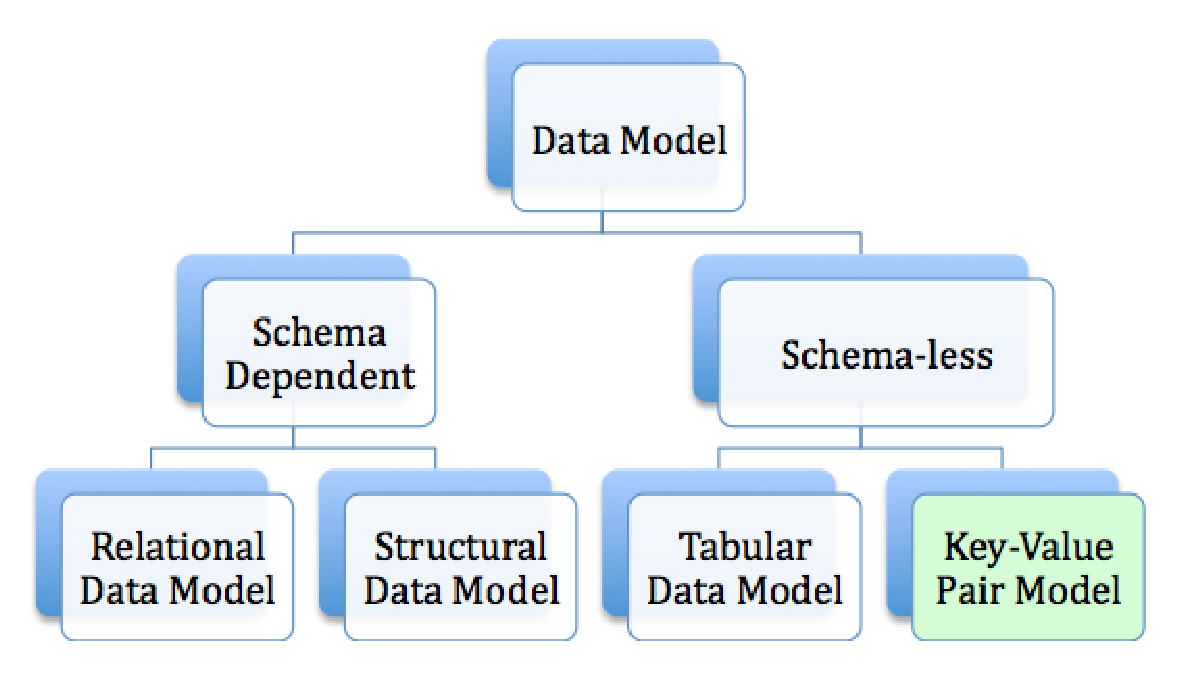
\includegraphics[scale=0.65]{../diagrams/taxonomy-data-model-modified}
  \caption{Data Model Taxonomy}
  \label{fig:taxonomy-data-model-modified}
\end{figure}

\subsection{Applicability and Recommendations}

This work can be used to evaluate data persisten in sensor networks in
different ways. The use of the data persistence taxonomies through this work
and guided both the evaluation and implementation of the data model using
mongoDB. In order to use the guidelines proposed by this work, one may first
determine the properties of the sensor network in question. Considering that
sensor devices produce streams of non-described data, the use of key-value
pairs data model did not require changes throughout different application
layers.

Focusing on the different layers of an application, consider the different
multi-tier application approaches where each layer implements a functionality
of the system such as the Model-View-Controler (MVC) \cite{sw-architectures}.
Usually, the use of traditional database systems and object-programming 
languages require ``data plumbing'' from the table relations from
the database system to the object instances. In order to implement all the
CRUD operations to a relational database without an ORM \cite{orm} offering,
the implementation of the data model potentially uses the Structured-Query
Language (SQL) for the problem of data plumbing, what results in a
tightly-coupled implementation. On the other hand, mongoDB eliminates the use
of an additional query language because it uses declarative approach on top of
the programming language drivers it support, decreasing the complexity of the
application.

Sensor networks with medium or large volumes of data are implemented nowadays
using clusters and parallel programming. Google's BigTable \cite{bigtable} uses
the principle of structured data in distributed tabular format, processing large
volumes of data using the MapReduce parallel approach \cite{map-reduce}. The
current version of mongoDB offers its first version of the MapReduce approach,
but it is still imature. However, it can be useful to process large amount of
data collected from sensor devices, or process historical data for any type of
analysis.

\subsection{Difficulties Experienced}
\label{sec:experiments-difficulties}

Particularly speaking about the learning curve, different situations
contributed to the success of the first experiments. The first problem to be
solved was the selection of the data model to be used during the technology
selection. Since relational database systems are the ``traditional'' way to
provide data persitence, the investigations started by creating a relational
model described in Chapter 5. Then, the technique using KVP data models in
relational databases were attempted without success. Only after reviewing the
technical article \cite{db-is-rdbs-dommed}, suggested the advisor of this 
work, the search for a database system that uses the KVP data model was
considered, and finally successfully implemented.

Since the technology is new, it brought new challenges regarding the usability
and user experience. The technology is relatively new and still under development,
many different bugs were be reproduced at random during the execution of
the experiments, and therefore, reports were sent to the open-source community
through various communication channels. To address this, the fastest way to
solve an issue was through the mongoDB's IRC channel located at the Freenode
server (www.freenode.org, channel mongodb). Second, the users group, located at
http://groups.google.com/group/mongodb-user also helped troubleshooting
problems.

Physical memory is limited and, for this reason, it may not be enough to run
the experiments for total workloads. In this case, the Java Virtual Memory was
totally consumed by one of the revisions of the experiments setup. Therefore, 
it was learned that large amount of data loads require different techniques to
manage data in memory accordingly, such as creating different object pools as
temporary caches for objects whose internal state are similar to others in the
JVM. Also, operations that involve writing in disk, such as during the bulk
``Create'' operations, may lead to different database performance. First, the
experiment seemed to stop inserting objects in one shard while it ran for over
2 minutes without inserting any documents. The reason was that the partition
was ``/home'', completely full, leading to the problem. The mongos cluster
header did not realize that it was the time to switch to another shard.
Similarly, any global ``Retreave'' operation on a cluster blocks all the
shards. For this reason, dividing the write from the read load was necessary in
order to decouple these two operations.

Also related to the difficulties of this work, mongoDB is not yet stable, and
therefore, harder to implement. The main production version of mongoDB is
is on version 1.1.4 at this time, while the shards support is still in alpha
version. For instance, different work-arounds were performed to have shards
experimented as described, but the execution was not successful.

To sum up, this chapter described the experimental results of the
implementation of a data persistence component for NetBEAMS, showing the
experiment results, the measurement results and finally the discussion about
the solution in general. The following section brings the conclusions and
future works for this report.
